\section{Trasformata di Fourier}
\lecture{4}{7 marzo 2024}

Nella soluzione generale abbiamo studiato esclusivamente funzioni periodiche con proprietà comode che sono spesso verificate nei sistemi fisici. Il secondo passo è studiare una funzione che descriva un effetto limitato nel tempo: possiamo immaginare che abbia un periodo \(T \to \infty \).

Consideriamo un intervallo di tempo ampio T tra \(-\frac{T}{2}\) e \(+\frac{T}{2}\) e risolviamo \(\hat{L} (x) = f(t)\). In questo intervallo, posso approssimare \(f(t)\) con una serie di Fourier detta \(f_s(t)\). Nell'intervallo, \(f_s(t)\to f(t)\). La serie di Fourier più comoda è la serie complessa.

\begin{figure}[H]
	\centering
	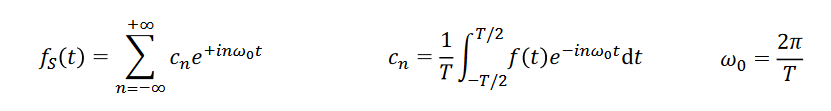
\includegraphics[width=0.8\textwidth]{screenshots/2024-03-07-09-20-30.png}
\end{figure}

Mi limito a funzioni continue, integrabili e con \(\int_{-\infty}^{\infty} \vert f(t) \vert  \,\mathrm{d}t \) finito.

\begin{figure}[H]
	\centering
	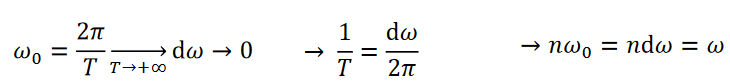
\includegraphics[width=0.8\textwidth]{screenshots/2024-03-07-09-23-47.png}
\end{figure}

La pulsazione \(\omega \) è una variabile continua, anche se è data dal prodotto di un numero intero n e un infinitesimo \(\mathrm{d} \omega  \). Sto operando un passaggio dal discreto al continuo. 

\begin{figure}[H]
	\centering
	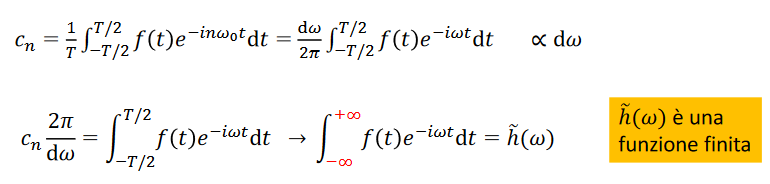
\includegraphics[width=0.8\textwidth]{screenshots/2024-03-07-09-28-07.png}
	\caption{Divido per \(\mathrm{d}\omega  \) per evitare che il secondo membro tenda a zero. Il risultato è una funzione continua e finita, ottenuta integrando su tutti i tempi (\(T \to \infty \) ). }
\end{figure}

\begin{figure}[H]
	\centering
	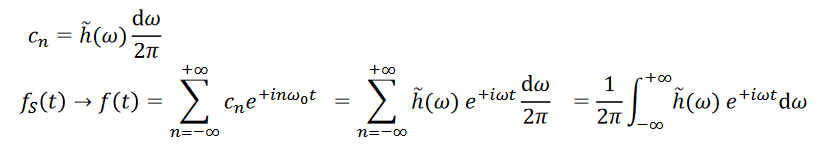
\includegraphics[width=0.8\textwidth]{screenshots/2024-03-07-09-29-55.png}
	\caption{Adesso che ho una dipendenza da \(\mathrm{d}\omega  \) posso trasformare la sommatoria in un integrale. Rappresentando tutti gli n rappresento tutte le \(\omega \).  }
\end{figure}

\begin{definition}
	[Trasformata di Fourier]
	Data una funzione continua, a modulo integrabile, definita sull'asse reale, si definisce trasformata di Fourier della funzione f(t):
	\[
		\widetilde{f}(\omega )=\int_{-\infty}^{\infty} f(t)e^{-i \omega t} \,\mathrm{d}t  
	\]
	\(\widetilde{f}(\omega ) \) descrive la componente di \(e^{i \omega t}\) nella funzione di partenza. La \(f(t)\) è rappresentabile come sovrapposizione continua di fasori:
	\begin{figure}[H]
		\centering
		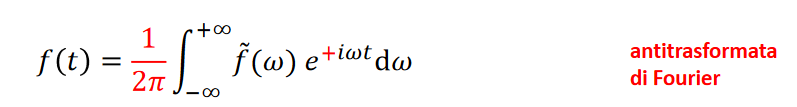
\includegraphics[width=0.8\textwidth]{screenshots/2024-03-07-09-36-07.png}
	\end{figure}   
\end{definition}

La differenza con la serie di Fourier è che nella trasformata di Fourier siamo passati al continuo, mentre nella serie avevamo delle pulsazioni discrete. Questo procedimento è del tutto generale. Analizziamo le proprietà della trasformata di Fourier. Sia \(\mathcal{F} \) l'operatore trasformata di Fourier:

\begin{itemize}
	
	\item \(\mathcal{F} \) è lineare:
	\begin{figure}[H]
		\centering
		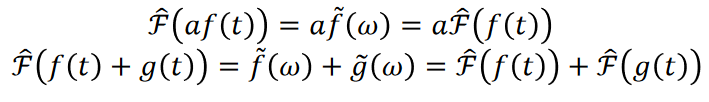
\includegraphics[width=0.8\textwidth]{screenshots/2024-03-07-09-40-06.png}
	\end{figure}
	
	\item Le derivate diventano moltiplicazioni, come già visto con i fasori:
	\begin{figure}[H]
		\centering
		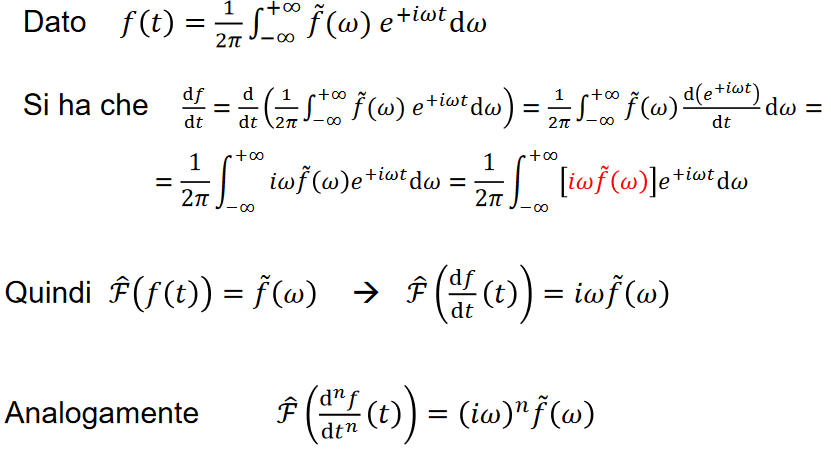
\includegraphics[width=0.8\textwidth]{screenshots/2024-03-07-09-41-51.png}
	\end{figure}
\end{itemize}

\subsection{Applicazione all'oscillatore armonico forzato}

Iniziamo applicando ad entrambi i membri della solita equazione la trasformata di Fourier.
\begin{figure}[H]
	\centering
	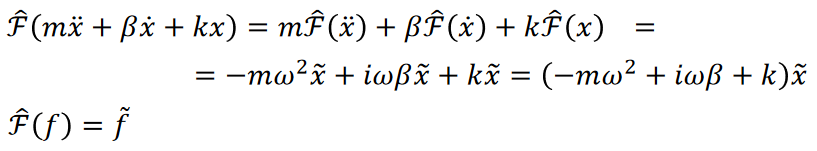
\includegraphics[width=0.8\textwidth]{screenshots/2024-03-07-09-46-30.png}
	\caption{Ottengo così un'uguaglianza fra le due trasformate. Applico la seconda proprietà della trasformata di Fourier per cui le derivate diventano moltiplicazioni. \(\widetilde{x} \) è la mia incognita. }
\end{figure}
\begin{figure}[H]
	\centering
	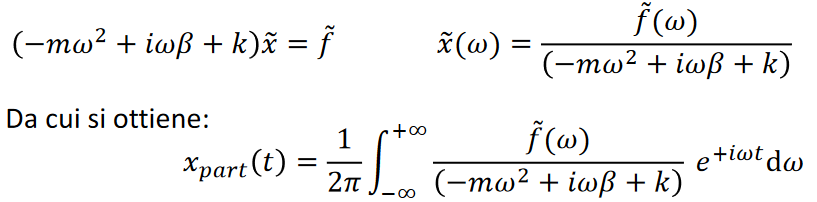
\includegraphics[width=0.8\textwidth]{screenshots/2024-03-07-09-48-28.png}
	\caption{Così ho risolto il problema nello spazio delle pulsazioni. Con l'antitrasformata di Fourier posso trovare la soluzione particolare nello spazio dei tempi.}
\end{figure}
Non è chiaramente un processo matematico semplice, ma con l'aiuto dei computer questi integrali sono facilmente risolvibili numericamente. Proseguiamo con alcune osservazioni:
\begin{enumerate}
	\item Le equazioni differenziali lineari si trasformano in polinomi in \(\omega \):
	\begin{figure}[H]
		\centering
		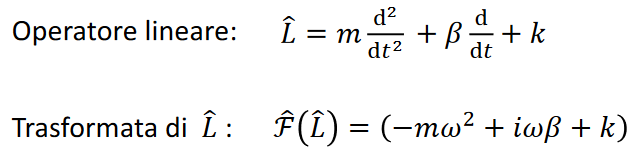
\includegraphics[width=0.8\textwidth]{screenshots/2024-03-07-09-51-21.png}
		\caption{Posso vedere la trasformata di Fourier anche come un operatore che agisce su altri operatori.}
	\end{figure}
	
	\item t e \(\omega \) sono variabili coniugate. La trasformata di Fourier non è necessariamente collegata al tempo, basta avere due variabili coniugate: ad esempio, posso fare la trasformata di Fourier anche di un segnale periodico nello spazio. \(\frac{\mathrm{d}}{\mathrm{d}t} \leftrightarrow i \omega   \), il primo agisce nello spazio delle \(f(t)\) e il secondo agisce nello spazio delle \(\widetilde{f}(\omega ) \).  
\end{enumerate}

\begin{note}
	[Diverse definizioni di trasformata di Fourier]
	La definizione della trasformata di Fourier può essere diversa. Noi non le useremo mai! L'importante è associare l'antitrasformata corretta in base alla definizione di trasformata che abbiamo usato. Alcuni esempi:
	\begin{figure}[H]
		\centering
		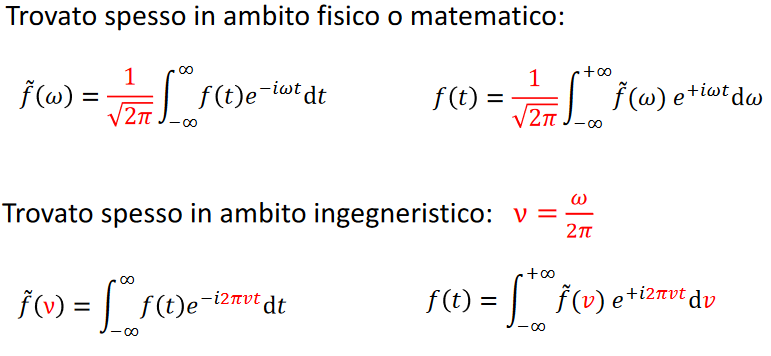
\includegraphics[width=0.8\textwidth]{screenshots/2024-03-07-09-57-28.png}
		\caption{La prima è fatta per una questione di simmetria. La seconda è comoda per utilizzare il concetto di frequenza, che agli ingegneri sembra più naturale del concetto di pulsazione.}
	\end{figure}
\end{note}

\chapter{Onde meccaniche}

Facciamo un riepilogo di cosa sono le onde:
\begin{itemize}
	
	\item Un'onda è una perturbazione che si propaga nello spazio, partendo da una condizione di "equilibrio"
	\item Per avere un'onda è necessario avere almeno una grandezza fisica che oscilla: onde scalari, vettoriali, tensoriali
	\item Le onde hanno una sorgente, che è un punto o una regione dello spazio da dove parte la perturbazione
	\item Le onde hanno una velocità con cui si propagano
	\item Possono trasportare informazione, energia, potenza, quantità di moto. Solo quelle quantistiche possono trasportare materia, le altre non trasportano materia.
	\item Le onde meccaniche richiedono un mezzo di propagazione.
\end{itemize}

\paragraph{Caratteristiche delle onde meccaniche} Le onde meccaniche, che sono la prima tipologia di onde che studieremo, hanno alcune caratteristiche generali:
\begin{itemize}
	
	\item Si propagano nei mezzi continui.
	\item Sono oscillazioni coerenti delle posizioni di elementi materiali.
	\item Possono essere unidimensionali (onde su corda tesa), bidimensionali (noi non le faremo, sono quelle su un tamburo o del mare) o nello spazio (onde sonore, vibrazioni, sismiche).
	\item Per queste onde si studia lo spostamento di un elemento infinitesimo di materiale, quindi sono onde vettoriali. Inizialmente noi le studieremo come onde scalari.
	\item Esistono due grandi categorie di onde meccaniche: onde trasversali e onde longitudinali. Per le prime la velocità dell'onda è in una certa direzione e il moto del mezzo meccanico è in direzione ortogonale a quella di propagazione (molla oscillata). Nelle onde longitudinali invece l'oscillazione è nella direzione di moto dell'onda (molla compressa).
\end{itemize}

\paragraph{Caratteristiche delle onde elettromagnetiche}
Le onde elettromagnetiche presentano delle differenze rispetto a quelle meccaniche:
\begin{itemize}
	
	\item Si propagano nel vuoto e nei mezzi continui
	\item Sono oscillazioni simultanee di campo elettrico e magnetico, sono particolari soluzioni delle equazioni di Maxwell
	\item Sono onde vettoriali e trasversali
	\item Nel vuoto si muovono sempre alla velocità della luce indipendentemente dal sistema di riferimento: origine della relatività ristretta!
\end{itemize}

La comodità delle onde meccaniche è che, propagandosi in un mezzo, esiste un sistema di riferimento privilegiato, ovvero il sistema in cui il mezzo è fermo.

\section{Onde su una corda}

\begin{figure}[H]
	\centering
	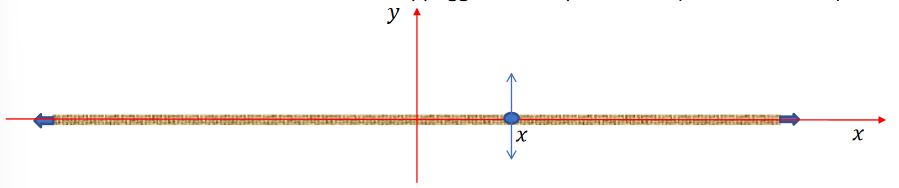
\includegraphics[width=0.8\textwidth]{screenshots/2024-03-07-10-29-38.png}
	\caption{Riferimento per lo studio delle onde trasversali su una corda.}
\end{figure}

La corda è elastica, uniforme, tesa e appoggiata su un piano liscio. La corda si può muovere nel piano xy. Per ora ci limitiamo allo studio dei casi in cui, preso un punto della corda a coordinata x, questo si possa muovere solo nella direzione y (quindi onde trasversali e non longitudinali). Devo studiare una funzione di due variabili che descriva i movimenti verticali della corda: \(\xi (x,t)\), detta onda o funzione d'onda. Se la corda è ferma, \(\xi (x,t) = 0 \forall x,t\). Questa è detta condizione di equilibrio. Nel caso di moti sulla corda, la derivata rispetto al tempo della funzione \(\xi \) è diversa da zero: \(\frac{\partial \xi (x,t)}{\partial t} \neq 0\) è la velocità verticale della corda in x.

\paragraph{Dinamica per la funzione \(\xi (x,t)\) } Consideriamo un tratto infinitesimo \(\mathrm{d} x \) di massa \(\mathrm{d} m \). La densità di massa sarà \(\frac{\mathrm{d}m}{\mathrm{d}x} 	\).

\begin{figure}[H]
	\centering
	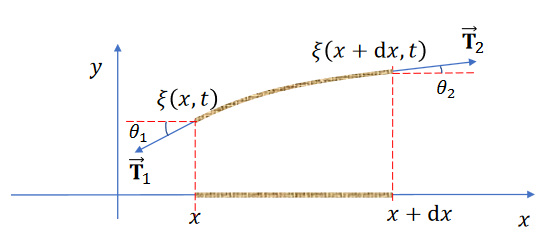
\includegraphics[width=0.8\textwidth]{screenshots/2024-03-07-10-36-23.png}
	\caption{Studio della dinamica di un tratto infinitesimo della corda.}
\end{figure}

Le tensioni nella corda sono dovute al pezzo di corda al di fuori del tratto \(\mathrm{d}x \). Le tensioni sono tangenti alla corda. L'equazione per la dinamica di questo tratto è \(\vec{T_1} +\vec{T_2} = \mathrm{d}m \vec{a} \). N.B: l'accelerazione è verticale, \(\vec{a} = a \hat{j} \). Posso assumere che \(a=\frac{\partial ^{2} \xi }{\partial t^{2} } \). Per semplificare la trattazione, mi riconduco al regime delle piccole oscillazioni: \(\theta _i \ll  1,\ \cos \theta _i \approx 1,\ \sin \theta _i \approx \tan \theta _i \approx \theta _i \).

\begin{figure}[H]
	\centering
	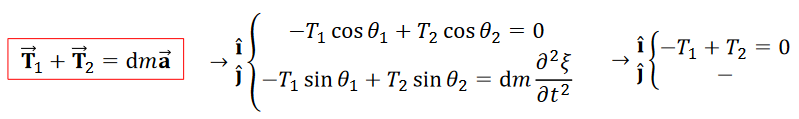
\includegraphics[width=0.8\textwidth]{screenshots/2024-03-07-10-41-03.png}
\end{figure}

Pongo \(T=T_1=T_2\). Ho verificato che il modulo tensione della corda è uguale in ogni verso (per le piccole oscillazioni). Osserviamo che \(\tan \theta _i = \frac{\partial \xi}{\partial x} \). Di conseguenza, \(\sin \theta _1 \approx \tan \theta _1= \frac{\partial \xi }{\partial x} \vert_x \) e \(\sin \theta _2 \approx \tan \theta _2 = \frac{\partial \xi }{\partial x}\vert_{x+\mathrm{d}x }  \).

\begin{figure}[H]
	\centering
	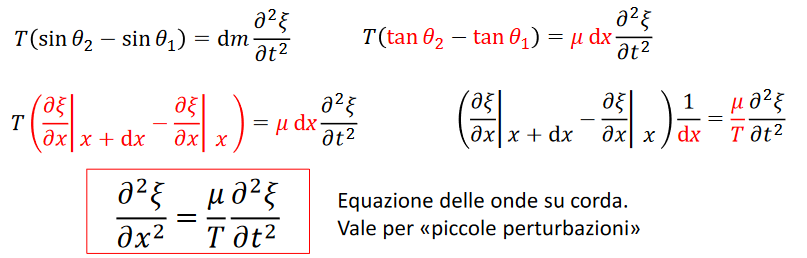
\includegraphics[width=0.8\textwidth]{screenshots/2024-03-07-10-47-36.png}
\end{figure}

L'equazione appena ricavata è molto importante. Per iniziare, considereremo casi in cui \(\mu \) è costante. È detta equazione di D'Alembert. Per ricordarci che \(\frac{\mu }{T}\) è una quantità positiva, la scriviamo come il quadrato di una quantità. Notiamo che ha le dimensioni dell'inverso di una velocità: \(\frac{\mu }{T} = \frac{1}{v^{2} } \to v=\sqrt{\frac{T}{\mu }} \). Dimensionalmente si vede che è effettivamente una velocità:
\begin{figure}[H]
	\centering
	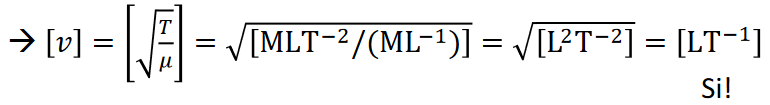
\includegraphics[width=0.8\textwidth]{screenshots/2024-03-07-10-54-11.png}
\end{figure}
L'equazione di D'Alembert è lineare, per cui vale il principio di sovrapposizione. Compaiono derivate seconde al primo grado:
\begin{equation}
	\label{eq:dalembert_1d}
	\frac{\partial^{2}  \xi }{\partial x^{2} } = \frac{1}{v^{2} }\frac{\partial ^{2} \xi }{\partial t^{2} } 
\end{equation}